%  LaTeX support: latex@mdpi.com 
%  For support, please attach all files needed for compiling as well as the log file, and specify your operating system, LaTeX version, and LaTeX editor.

%=================================================================
% UNCOMMENT THE FOLLOWING LINE FOR PRODUCTION WITH mdpi.cls:
\documentclass[journal,article,submit,pdftex,moreauthors]{Definitions/mdpi} 

%=================================================================
% MDPI internal commands
\firstpage{1} 
\makeatletter 
\setcounter{page}{\@firstpage} 
\makeatother
\pubvolume{1}
\issuenum{1}
\articlenumber{0}
\pubyear{2025}
\copyrightyear{2025}
\datereceived{ } 
\daterevised{ } 
\dateaccepted{ } 
\datepublished{ } 
\hreflink{https://doi.org/} 

%=================================================================
% Add packages and commands here.
\usepackage{amsmath}
\usepackage{amssymb}
\usepackage{booktabs} 
\usepackage{multirow}
\usepackage{graphicx}
\usepackage{algorithm}
\usepackage{algorithmic}
\usepackage{bm} 
\usepackage{url}
\usepackage{float}

%=================================================================
% Full title of the paper (Capitalized)
\Title{Adaptive Ensemble Weight Optimization for Natural Gas Consumption Forecasting: A Hybrid Stochastic-Deep Learning Framework Applied to the Czech Market}

% Authors
\Author{Vojtěch Vávra $^{1}$ and Josef Jablonsky $^{1}$*}

% Affiliations
\address{%
$^{1}$ \quad Department of Econometrics, Prague University of Economics and Business, Czech Republic}

% Contact information
\corres{Correspondence: jablon@vse.cz}

% Abstract
\abstract{
\textbf{Problem:} The transition towards data-driven energy management necessitates advanced predictive frameworks capable of handling the non-linear and non-stationary nature of natural gas consumption. Traditional static models struggle to adapt to rapid regime shifts in liberalized markets.\\
\textbf{Method:} This study proposes a convex ensemble weight optimization framework to address this challenge. Moving beyond simple model averaging, we formulate the ensemble weighting problem as a constrained convex optimization task on the unit simplex. We utilize the Frank-Wolfe algorithm (Conditional Gradient) to dynamically optimize the weights of a heterogeneous set of base learners, including SARIMAX, XGBoost, N-HiTS, and Temporal Fusion Transformers (TFT).\\
\textbf{Results:} Our results on the Czech gas market dataset demonstrate that this mathematically rigorous approach (MAPE 4.25\%) significantly outperforms both individual state-of-the-art models (N-HiTS 5.31\%) and static averaging (6.74\%). While the accuracy gain over greedy ensemble selection is marginal, the proposed convex formulation offers superior stability and interpretability, which are critical for operational deployment.
}

% Keywords
\keyword{Convex Optimization; Frank-Wolfe Algorithm; Ensemble Learning; Deep Learning; Machine Learning; Natural Gas Forecasting;}

%%%%%%%%%%%%%%%%%%%%%%%%%%%%%%%%%%%%%%%%%%
\begin{document}

%%%%%%%%%%%%%%%%%%%%%%%%%%%%%%%%%%%%%%%%%%
\section{Introduction}

The accurate forecasting of natural gas consumption is a cornerstone of energy security and economic efficiency, particularly in countries with high import dependence and seasonal demand variability like the Czech Republic. The liberalization of energy markets has shifted the focus towards data-driven decision-making, where the ability to predict daily demand fluctuations directly impacts the financial stability of market participants \citep{ref_ote}. In the context of the European energy crisis and the transition to renewable sources, the volatility of consumption patterns has increased, rendering traditional static forecasting models insufficient \citep{ref_mdpi_energies_1}. As highlighted by \citep{ref_potocnik}, static models fail to capture the concept drift in residential consumption, necessitating adaptive forecasting frameworks.

Current literature largely focuses on the development of increasingly complex individual architectures, ranging from Gradient Boosting Machines (GBM) \citep{ref_xgboost, ref_lgbm} to Recurrent Neural Networks (RNN) \citep{ref_mdpi_math_1}. However, the "No Free Lunch" theorem implies that no single model is universally superior across all temporal regimes. While ensemble learning offers a pathway to mitigate this limitation, standard approaches often rely on simple averaging or heuristic meta-learners that lack theoretical convergence guarantees. This paper addresses this gap by shifting the research focus from the development of individual predictors to the \textit{operational research} problem of optimal forecast combination.

The primary hypothesis of this study is that the daily prediction task can be modeled as a decision-making process where a meta-learner dynamically assigns weights to a portfolio of diverse algorithms. We posit that formulating this problem as a constrained convex optimization task on the unit simplex provides a regularization effect that significantly enhances stability compared to unconstrained or greedy approaches. Unlike "black-box" stacking methods, our proposed framework offers mathematical transparency, where the derived weights reflect the instantaneous reliability of each base learner. This formulation bridges the gap between purely data-driven Machine Learning ensembles and the rigorous constraint satisfaction of Operations Research. By mapping the forecasting problem onto the unit simplex, we substitute heuristic "tuning" with geometrical convergence guarantees.

The contribution of this study is threefold:
\begin{itemize}
    \item \textbf{Mathematical Formulation:} We frame the ensemble weighting problem as a constrained convex optimization task on a simplex, minimizing a regularized loss function that reflects the asymmetry of balancing costs \citep{ref_boyd}.
    \item \textbf{Algorithmic Solution:} We apply the Frank-Wolfe algorithm \citep{ref_fw_jaggi} and Ensemble Selection methods \citep{ref_caruana} to solve this optimization problem efficiently in a rolling-window production environment.
    \item \textbf{Empirical Validation:} We provide a comprehensive validation on real-world Czech gas consumption data. Crucially, we conduct an ablation study to quantify the contribution of each component of the ensemble and rigorously justify the choice of hyperparameters based on the physical properties of the natural gas market.
\end{itemize}

The remainder of this paper is organized as follows: Section 2 reviews the state-of-the-art, identifying the research gap in theoretically grounded ensemble methods. Section 3 details the proposed methodology, providing physical justifications for the chosen parameters. Section 4 presents the empirical results, including a detailed ablation study. Section 5 discusses the operational implications, and Section 6 concludes the work.

%%%%%%%%%%%%%%%%%%%%%%%%%%%%%%%%%%%%%%%%%%
\section{Literature Review}

The forecasting of energy consumption has undergone a paradigm shift from traditional econometric approaches to advanced artificial intelligence methods. This section reviews the evolution of these methodologies, summarizing their contributions and limitations in the context of natural gas markets. To provide a clear positioning of our work, we present a comparative analysis of state-of-the-art approaches in Table \ref{tab:lit_review}.

\subsection{Statistical and Machine Learning Approaches}
Historically, statistical linear models such as ARIMA and its seasonal variants (SARIMAX) were the industry standard. However, forecasting natural gas consumption involves capturing complex non-linear dependencies on meteorological factors, which linear models often fail to address adequately. As noted by \citep{ref_mdpi_energies_1}, methods like Multivariate Adaptive Regression Splines (MARS) have been proposed to handle these non-linearities better than traditional regression. Subsequently, machine learning algorithms such as Support Vector Regression (SVR) and Random Forests gained prominence. \citep{Dudek2021} demonstrated the effectiveness of Random Forest for short-term load forecasting, highlighting its robustness to non-stationarity.

\subsection{Deep Learning and Transformer Models}
In recent years, Deep Learning has achieved state-of-the-art results. Long Short-Term Memory (LSTM) networks are widely used to model temporal sequences \citep{ref_mdpi_math_1}. More recently, Transformer-based architectures have revolutionized the field. The Temporal Fusion Transformer (TFT) \citep{ref_tft} introduces a multi-head attention mechanism combined with variable selection networks. Another significant development is N-HiTS \citep{ref_nhits}, which reduces computational complexity using hierarchical blocks.

\subsection{Ensemble Learning Taxonomy}
Ensemble methods generally fall into three categories: Bagging/Boosting (e.g., XGBoost \citep{ref_xgboost}), Meta-Learning/Stacking, and Convex Weight Optimization. While Bagging and Stacking are powerful, they often lack interpretability. Our work adopts Convex Weight Optimization, applying the Frank-Wolfe algorithm to dynamically optimize weights on a unit simplex.

It is important to note that optimization algorithms have found broader applications in machine learning beyond simple weighting. Techniques such as Genetic Algorithms (GA) and Particle Swarm Optimization (PSO) have been extensively used for feature selection and hyperparameter tuning in energy forecasting \citep{ref_mdpi_energies_1}. However, these meta-heuristic approaches often lack convergence guarantees and require tuning of their own parameters. In contrast, convex optimization methods, such as the Frank-Wolfe algorithm used in this study, offer theoretical guarantees of convergence to a global optimum (for convex objectives) and are parameter-free regarding step-size selection in their standard form \citep{ref_fw_jaggi}. This distinction is crucial for building transparent and reliable decision-support systems for critical infrastructure.

\newcolumntype{L}[1]{>{\raggedright\let\newline\\\arraybackslash\hspace{0pt}}p{#1}}

\begin{table}[H]
\caption{Comparative analysis of related works in energy forecasting. (SOTA = State-of-the-Art).}
\label{tab:lit_review}
\centering
\scriptsize % Ještě menší písmo pro jistotu
\setlength{\tabcolsep}{2pt} % Minimální okraje uvnitř buněk
\resizebox{\textwidth}{!}{
% Součet šířek sloupců je optimalizován pro A4
\begin{tabular}{L{1.5cm} L{2.5cm} L{3.2cm} L{3.5cm} L{3.5cm}}
\toprule
\textbf{Category} & \textbf{References} & \textbf{Methodology} & \textbf{Key Advantages} & \textbf{Limitations} \\
\midrule
\multirow{5}{=}{Statistical} 
 & Taylor and Letham \citep{ref_prophet} & Prophet (Additive Model) & Handles missing data, outliers, and holidays well. & Fails to capture complex non-linear interactions. \\
 & Smajla et al. \citep{ref_smajla} & Statistical Distribution Analysis & Effective use of smoothed temperature ($T_{eff}$). & Limited by simplified physical assumptions. \\
 & Nalcaci et al. \citep{ref_mdpi_energies_1} & MARS, CMARS & Modeling of non-linearities in gas consumption. & Computational complexity in high dimensions. \\
 & Box and Jenkins & ARIMA / SARIMAX & Theoretical interpretability, seasonality handling. & Linear assumption limits accuracy in volatile markets. \\
\midrule
\multirow{4}{=}{Machine Learning} 
 & Chen and Guestrin \citep{ref_xgboost} & XGBoost & Scalability, sparsity awareness, SOTA for tabular data. & Requires extensive hyperparameter tuning. \\
 & Svoboda et al. \citep{ref_svoboda} & Smart Meter Data Mining & Insights from large-scale granular data collection. & Requires high-quality, dense historical data. \\
 & Dudek \citep{Dudek2021} & Random Forest & Robust to overfitting, handles non-stationarity. & Poor extrapolation outside training range. \\
\midrule
\multirow{5}{=}{Deep Learning \& Hybrid} 
 & Lim et al. \citep{ref_tft} & Temporal Fusion Transformers & Interpretable attention mechanisms, multi-horizon. & High computational resource requirements. \\
 & Zhao et al. \citep{ref_zhao} & Hybrid EL-VMD-Transformer & State-of-the-art accuracy by combining ensembles and DL. & Complex architecture, hard to deploy operationally. \\
 & Panapakidis and Dagoumas \citep{ref_panapakidis} & Wavelet + GA-ANFIS & Hybrid approach handling signal non-stationarity. & High complexity of the multi-stage pipeline. \\
 & Li and Sun \citep{ref_li_emlp} & EMLP (Adaptive MLP) & Adaptive weight correction within NN ensemble. & Weights optimized heuristically, not globally convex. \\
\midrule
\multirow{4}{=}{Ensemble Optimiz.} 
 & Marziali et al. \citep{ref_marziali} & Countrywide Ensembling & Proves ensembles outperform base learners (Italy). & Limited to standard averaging or simple regression. \\
 & Zhang et al. \citep{ref_mdpi_energies_2} & Dynamic Weighting & Adapts to time-varying model performance. & Heuristic weighting often lacks theoretical proof. \\
 & Caruana et al. \citep{ref_caruana} & Ensemble Selection & Greedy optimization, creates robust ensembles. & Can get stuck in local optima. \\
 & \textbf{This Study} & \textbf{Convex Optimization (FW)} & \textbf{Global convergence, sparsity, projection-free.} & \textbf{Requires convexity of the loss function.} \\
\bottomrule
\end{tabular}
}
\end{table}

Recent hybrid approaches, such as the EL-VMD-Transformer-ResLSTM proposed by \citep{ref_zhao}, demonstrate that combining tree-based ensembles with deep learning yields superior results. Similarly, \citep{ref_marziali} confirmed on Italian data that ensemble strategies consistently outperform individual predictors.

Despite the efficacy of individual models, the "No Free Lunch" theorem suggests that no single model performs best under all conditions.

As illustrated in Table \ref{tab:lit_review}, a significant gap exists in current methodologies. While deep learning models (TFT, N-HiTS) offer high accuracy, they suffer from opacity and high resource demands. Conversely, statistical models offer interpretability but lack the capacity to model complex non-linearities. Most existing ensemble approaches rely on heuristic weighting or greedy selection, which do not guarantee global optimality. Our study fills this gap by proposing a \textit{convex optimization framework} that combines the diverse strengths of these base learners. By mathematically guaranteeing convergence on the unit simplex, we offer a solution that is both interpretable (like statistical models) and high-performing (like deep learning ensembles), directly addressing the limitations identified in prior works.

%%%%%%%%%%%%%%%%%%%%%%%%%%%%%%%%%%%%%%%%%%
\section{Materials and Methods}

To address the non-stationarity of gas consumption, we propose a modular Three-Layer Ensemble Framework. This structure ensures a clear separation of concerns between prediction generation, temporal adaptation, and weight optimization.

\subsection{Layer 1: Base Learners (The Prediction Pool)}
The first layer consists of a heterogeneous library of 15 algorithms. Diversity is critical for ensemble success; therefore, we deliberately selected models with distinct inductive biases, ranging from classical econometric methods to deep learning architectures. The complete set of base learners is detailed below.

\subsubsection{Tree-Based Ensemble Methods}
Gradient boosting decision trees represent the state-of-the-art for tabular data. We employed four distinct implementations to maximize diversity:
\begin{itemize}
    \item \textbf{XGBoost:} A scalable implementation of gradient boosting that utilizes a sparsity-aware algorithm for handling sparse data and a weighted quantile sketch for approximate tree learning \citep{ref_xgboost}.
    \item \textbf{LightGBM:} A gradient boosting framework that uses tree-based learning algorithms. It is designed to be distributed and efficient, utilizing a leaf-wise growth strategy rather than the level-wise strategy used by other boosting algorithms \citep{ref_lgbm}.
    \item \textbf{CatBoost:} A high-performance library that handles categorical features automatically. It employs ordered boosting to overcome prediction shift, a common issue in traditional gradient boosting algorithms \citep{ref_catboost}.
    \item \textbf{ExtraTrees (Extremely Randomized Trees):} Unlike boosting methods, this is a bagging method similar to Random Forest but with more randomness in the split selection. This randomness helps to reduce variance and makes the model robust to noise.
\end{itemize}

\subsubsection{Deep Learning Architectures}
Neural networks are employed to capture complex, non-linear temporal dependencies that traditional models might miss:
\begin{itemize}
    \item \textbf{Temporal Fusion Transformers (TFT):} An attention-based architecture that combines high-performance multi-horizon forecasting with interpretable insights into temporal dynamics. It utilizes variable selection networks and gating mechanisms to learn relationships at different time scales \citep{ref_tft}.
    \item \textbf{N-HiTS (Neural Hierarchical Interpolation for Time Series):} A model that solves the forecasting problem by using multi-rate signal sampling and hierarchical interpolation. It is designed to capture long-range dependencies efficiently without the computational cost of standard Transformers \citep{ref_nhits}.
    \item \textbf{Long Short-Term Memory (LSTM):} A type of recurrent neural network (RNN) capable of learning order dependence in sequence prediction problems. Our implementation consists of a stacked LSTM with two layers to model the sequential nature of gas demand \citep{ref_mdpi_math_1}.
    \item \textbf{NeuralProphet:} A hybrid framework based on PyTorch that combines the interpretability of statistical models with the scalability of deep learning. It models seasonality and autoregression using neural network modules.
\end{itemize}

\subsubsection{Statistical and Econometric Models}
To ensure the ensemble is grounded in established statistical theory, we included:
\begin{itemize}
    \item \textbf{SARIMAX:} The Seasonal AutoRegressive Integrated Moving Average with exogenous factors model. It explicitly models the seasonal components and the impact of external variables like temperature.
    \item \textbf{ARX (Robust):} An AutoRegressive model with exogenous variables. This variant is implemented to focus purely on linear dependencies between past consumption and current weather drivers.
    \item \textbf{Prophet:} An additive regression model developed by Meta. It works best with time series that have strong seasonal effects and several seasons of historical data. It is robust to missing data and shifts in the trend \citep{ref_prophet}.
\end{itemize}

\subsubsection{Classical Machine Learning}
Finally, we diversified the pool with classical regression and instance-based algorithms:
\begin{itemize}
    \item \textbf{Support Vector Regression (SVR):} A regression method that finds a hyperplane in an N-dimensional space. It is effective in high-dimensional spaces and robust against overfitting in cases where the number of dimensions is greater than the number of samples.
    \item \textbf{K-Nearest Neighbors (KNN):} A non-parametric method that predicts consumption based on the average of the $k$ most similar historical days in the feature space.
    \item \textbf{ElasticNet:} A linear regression model that combines L1 and L2 priors as regularizers. It is particularly useful when there are multiple correlated features.
    \item \textbf{Bayesian Ridge:} A probabilistic approach to linear regression that introduces a prior probability distribution over the model parameters, providing a robust alternative to standard linear regression.
\end{itemize}

Each model $i$ generates an independent forecast $\hat{y}_{i,t}$.

\subsection{Layer 2: Temporal Weighting Strategy}
The second layer constitutes the adaptive "memory" of the system, addressing the challenge of concept drift where the statistical properties of the target variable change over time. In energy markets, such shifts are frequent due to seasonality, policy changes, or sudden geopolitical events. Standard ensemble methods often assume that all historical data points are equally relevant ($\omega_t = 1$), which leads to slow adaptation rates in non-stationary environments.

To mitigate this, we introduce a temporal weighting mechanism directly into the convex loss function. The objective is to minimize a weighted sum of errors over the historical window $H$. Formally, the optimization problem is defined as:
\begin{equation}
    \min_{\mathbf{w} \in \Delta_N} \sum_{t=1}^H \omega_t \cdot \mathcal{L}\left(y_t, \sum_{i=1}^N w_i \hat{y}_{i,t}\right)
\end{equation}

%\begin{align}
%    \min_{\mathbf{w}} \quad & f(\mathbf{w}) = \frac{1}{H} \sum_{t=1}^H \mathcal{L}\left(y_t, \sum_{i=1}^N w_i %\hat{y}_{i,t}\right) \\
%    \text{s.t.} \quad & \sum_{i=1}^N w_i = 1, \quad w_i \ge 0 \quad (\mathbf{w} \in \Delta_N)
%\end{align}

where $\omega_t$ represents the importance weight of observation $t$, $y_t$ is the actual consumption, and $\mathcal{L}$ is the loss function (typically Mean Squared Error for convex stability).

We critically evaluate two distinct weighting kernels to determine the optimal adaptation strategy:
\begin{itemize}
    \item \textbf{Exponential Decay:} A continuous forgetting factor commonly used in online learning, defined as $\omega_t = \lambda^{H-t}$, where $\lambda \in (0, 1]$ is the decay rate. While theoretically sound, this method can be overly aggressive in discarding useful information from the recent past if $\lambda$ is too small.
    \item \textbf{Recency-Weighted Heuristic:} We formally define this method through a Weighted Loss Function where weights $\omega_t$ are adjusted to reflect temporal relevance. Specifically, observations $t \in T_{recent}$ (the most recent week) are assigned a weight $\omega_t = 3$, while older observations retain $\omega_t = 1$.
    
    \textit{Justification of Parameter Choice:} The selection of the weighting factor $\omega_{high}=3$ and the window length is not arbitrary but grounded in the meteorological dynamics of Central Europe. Synoptic weather systems (cyclones/anticyclones) which drive heating demand typically persist for 3 to 5 days. By weighing the most recent week significantly higher, the model captures the inertia of the current weather regime (e.g., a cold snap) while the baseline history prevents overfitting to measurement noise. This approximates a Bayesian prior where the "current regime" is three times more informative than the "climatological average." The weighting factor $\omega_{high}=3$ is adopted as an expert-standard value based on domain knowledge from a Czech energy company.
\end{itemize}
The choice of the discrete heuristic is motivated by the "shock" nature of gas consumption anomalies (e.g., a sudden cold front), where the most recent days are significantly more predictive of the immediate future than a smooth exponential decay would suggest.

\subsection{Layer 3: Ensemble Optimizer (Frank-Wolfe)}
The third layer is the computational engine of the framework, tasked with solving the constrained convex optimization problem to find the optimal weight vector $\mathbf{w}$. We employ the Frank-Wolfe algorithm (Conditional Gradient), a projection-free first-order optimization method.

The choice of Frank-Wolfe over standard Projected Gradient Descent (PGD) is driven by two key theoretical advantages relevant to our domain:
\begin{itemize}
    \item \textbf{Computational Efficiency (Projection-Free):} In standard PGD, every iteration requires a Euclidean projection of the weight vector onto the probability simplex $\Delta_N$ to satisfy the constraints $\sum w_i = 1$ and $w_i \ge 0$. This projection operation typically has a complexity of $\mathcal{O}(N \log N)$. In contrast, Frank-Wolfe replaces the projection with a Linear Minimization Oracle (LMO), which solves a linear sub-problem over the simplex. For the unit simplex, this LMO is trivial and equivalent to finding the index of the minimum gradient component, reducing the complexity to $\mathcal{O}(N)$.
    \item \textbf{Sparsity of Solutions:} Frank-Wolfe updates the solution by iteratively moving towards a vertex of the simplex (a single base learner). After $K$ iterations, the solution is a convex combination of at most $K+1$ vertices. This property naturally encourages sparsity, effectively selecting a compact subset of the most relevant models from the pool of 15 base learners, thereby improving interpretability and reducing overfitting.
\end{itemize}

The algorithm operates by linearizing the objective function at the current iterate and moving towards the minimizer of this linear approximation. The detailed procedure is outlined in Algorithm \ref{alg:fw}.

\begin{algorithm}[H]
\caption{Frank-Wolfe for Ensemble Weights Optimization}
\label{alg:fw}
\begin{algorithmic}[1]
\STATE \textbf{Inputs:} 
\begin{itemize}
    \item Matrix of predictions $\mathbf{P} \in \mathbb{R}^{H \times N}$
    \item Vector of actual values $\mathbf{y} \in \mathbb{R}^H$
    \item Sample weights $\bm{\omega} \in \mathbb{R}^H$
\end{itemize}
\STATE \textbf{Parameters:} 
\begin{itemize}
    \item $K$: Number of iterations (set to 500)
    \item $\epsilon$: Tolerance parameter
\end{itemize}
\STATE \textbf{Output:} Optimized weight vector $\mathbf{w}^{(K)} \in \Delta_N$
\STATE \textbf{Initialization:} Start with uniform weights $\mathbf{w}^{(0)} = [1/N, \dots, 1/N]^T$
\FOR{$k = 0 \dots K$}
    \STATE Compute gradient $\nabla f(\mathbf{w}^{(k)})$ based on weighted loss
    \STATE \textit{Linear Minimization Oracle (LMO):} Find vertex $\mathbf{s}^{(k)}$ with smallest gradient:
    \STATE $\mathbf{s}^{(k)} \leftarrow \arg\min_{\mathbf{s} \in \Delta_N} \langle \mathbf{s}, \nabla f(\mathbf{w}^{(k)}) \rangle$
    \STATE Calculate step size $\gamma \leftarrow \frac{2}{k+2}$
    \STATE Update weights: $\mathbf{w}^{(k+1)} \leftarrow (1-\gamma)\mathbf{w}^{(k)} + \gamma \mathbf{s}^{(k)}$
\ENDFOR
\RETURN $\mathbf{w}^{(K)}$
\end{algorithmic}
\end{algorithm}

To rigorously validate the efficacy of the proposed Frank-Wolfe approach, we benchmark it against three distinct classes of optimization strategies implemented within the same framework:
\begin{itemize}
    \item \textbf{Non-Negative Least Squares (NNLS):} This represents the exact analytical solution to the convex optimization problem $\min \|\mathbf{Pw} - \mathbf{y}\|_2^2$ subject to $w_i \ge 0$. While NNLS provides the theoretically optimal solution for the training set, it often lacks regularization, leading to overfitting in high-noise environments compared to the iterative regularization of Frank-Wolfe.
    \item \textbf{Ensemble Selection (Greedy Optimization):} A discrete heuristic proposed by \citep{ref_caruana}. Instead of solving for continuous weights, this method iteratively adds the model that minimizes the ensemble's error to the pool. It serves as a robust baseline that avoids the complexities of quadratic programming but may get trapped in local minima due to its greedy nature.
    \item \textbf{Contextual Bandits (LinUCB):} To contrast our batch-based rolling window approach with online learning, we implemented a Linear Upper Confidence Bound (LinUCB) algorithm. Here, an agent selects a model at each time step based on the current context (weather features), treating the forecast error as a negative reward. This tests whether a fully online, context-aware selection strategy outperforms the convex weighting of a portfolio.
\end{itemize}

A key computational advantage over Projected Gradient Descent is that the Linear Minimization Oracle (LMO) naturally returns a vertex of the simplex, eliminating the need for computationally expensive projection steps.

\subsubsection{Theoretical Considerations on Loss Functions}

We selected the Mean Absolute Percentage Error (MAPE) as the primary evaluation metric because it aligns with the financial incentives of the gas market. Balancing penalties charged by the Market Operator (OTE) are typically proportional to the deviation relative to the nomination size, making a percentage-based metric more financially relevant than the Absolute Error (MAE). Furthermore, the penalty structure is often progressive; large deviations from the nominated schedule incur disproportionately higher unit costs than minor fluctuations. Consequently, the forecasting objective must aggressively penalize large errors to minimize financial risk, prioritizing the avoidance of extreme outliers over small, noise-level improvements.

While the Frank-Wolfe algorithm is theoretically grounded for smooth convex functions (like MSE), we extend its application to the Mean Absolute Percentage Error (MAPE), which is the industry standard in energy trading.
This introduces two theoretical nuances:
\begin{itemize}
    \item \textbf{Convexity:} The MAPE function $f(\mathbf{w}) = \frac{1}{H}\sum |\frac{y_t - \hat{y}_t(\mathbf{w})}{y_t}|$ is convex on the domain of weights $\mathbf{w}$ as long as the actual values $y_t$ are strictly positive. This consistency with convex optimization theory is supported by \citep{ref_mape_theory}, who formally proved that the expected MAPE risk is a convex function of model predictions for strictly positive targets (ensuring the existence of a global minimum), although it is not strictly convex.
    \item \textbf{Differentiability:} Unlike MSE, the absolute value function is not differentiable at zero (where prediction equals actual). However, in a continuous forecasting domain, the probability of the error being exactly zero is negligible. For practical optimization, we utilize sub-gradients or smooth approximations (e.g., Huber loss or Log-Cosh) where strict differentiability is required. Our empirical results demonstrate that the standard Frank-Wolfe update rule converges stably even with the non-smooth MAPE objective, consistent with recent findings on subgradient methods for non-smooth convex optimization \citep{ref_fw_jaggi}.
    \item \textbf{Differentiability and Stability:} Theoretical concerns regarding the singularity of MAPE at zero are mitigated by the domain properties. Descriptive statistics of the target variable covering the extensive 9-year history (N=3379) confirm the complete absence of zero values. The target variable remains strictly non-zero (empirically confirmed minimum magnitude $> 10^5$), ensuring that the MAPE metric remains numerically stable and differentiable almost everywhere throughout the optimization landscape.
\end{itemize}


\subsection{Data Engineering Pipeline}
The primary dataset consists of daily gas consumption series in the Czech Republic \citep{ref_ote} combined with weather data from the ERA5 reanalysis model \citep{ref_openmeteo}. A critical preprocessing step is the calculation of Effective Temperature ($T_{eff}$), which accounts for the thermal inertia of buildings:
\begin{equation}
    T_{eff, t} = 0.5 \cdot T_t + 0.5 \cdot T_{eff, t-1}
\end{equation}
where $T_t$ is the daily mean air temperature and $T_{eff, t-1}$ is the effective temperature of the previous day. This recursive filter smooths out rapid temperature fluctuations that do not immediately impact building heating demand. The utility of such temperature smoothing for reducing forecasting errors has been empirically validated by \citep{ref_smajla} on European gas distribution networks.

Beyond temperature transformations, we constructed a comprehensive feature set to capture the multiscale seasonality and autoregressive nature of gas consumption. The feature engineering process, implemented in Python, resulted in the following categories of predictors:
\begin{itemize}
    \item \textbf{Calendar Features:} To capture human-driven cycles, we generated boolean flags for weekends and public holidays specific to the Czech Republic. We also distinguished standard working days from non-working days. To model annual seasonality continuously, we employed cyclical encoding, transforming the day of the year into sine and cosine components.
    \item \textbf{Lagged Variables:} Autoregressive features are crucial for time-series forecasting. We included consumption lags corresponding to the previous day ($t-1$), two days prior ($t-2$), one week ($t-7$), and two weeks ($t-14$). These lags capture the immediate dependency and the strong weekly periodicity inherent in energy consumption data.
    \item \textbf{Meteorological Interactions:} In addition to effective temperature, we utilized raw air temperature, apparent temperature, and wind speed. For each of these meteorological variables, we generated lagged features (1-day and 2-day lags) and rolling window statistics (3-day and 7-day moving averages). These rolling features help the models distinguish between short-term weather shocks and longer-term climatic trends.
\end{itemize}

\subsubsection{Data Partitioning}
To ensure a robust evaluation aligned with the regulatory "Gas Year" structure, the dataset was chronologically partitioned into three subsets:

\begin{itemize}
    \item \textbf{The Training Set} covers the extensive historical period from July 1, 2016, to September 30, 2024. This allows the base learners to capture long-term seasonal patterns and structural dependencies over multiple years.
    
    \item \textbf{The Validation Set} (October 1, 2024 -- November 30, 2024) was selected to simulate a production environment where model recalibration prioritizes the most recent market regime. While the internal parameters are learned from the full history, hyperparameter tuning was deliberately restricted to this immediate pre-test period. This design choice ensures that the model's sensitivity is calibrated to the current onset of the heating season, rather than averaging performance across older, potentially irrelevant historical regimes (e.g., pre-energy crisis years). The use of the TPE algorithm (Hyperopt) ensures efficient convergence even within this focused validation window.
    
    \item \textbf{The Test Set} spans the remainder of the gas year (December 1, 2024 -- September 30, 2025), providing a strictly out-of-sample evaluation across the full winter peak and the subsequent spring/summer decline.
\end{itemize}

Although limited to a single gas year, this period represents a robust climatological stress test. Meteorological analysis, grounded in the climatological standards of the Market Operator \citep{ref_ote}, confirms that the test set encompasses significant temperature anomalies, fluctuating both above and below the 30-year normal. The data includes episodes of deep freezing events typical of continental winters, as well as unseasonably warm spells, effectively validating the model's adaptability to rapid regime shifts within a single heating season.

\subsection{Experimental Setup and Feasibility Testing}
The computational framework was developed within the Python 3.11 ecosystem, leveraging a suite of specialized libraries to ensure robust data processing and modeling. The data manipulation and feature engineering pipelines relied on \texttt{pandas} and \texttt{numpy} for efficient time-series handling, while \texttt{scikit-learn} provided the foundation for preprocessing (scaling) and evaluation metrics. The deep learning models (TFT, N-HiTS, LSTM) were implemented using \texttt{PyTorch} and the high-level API of \texttt{PyTorch Forecasting}, which facilitates the handling of complex temporal covariates. Conversely, the gradient boosting variants utilized their respective native libraries (\texttt{xgboost}, \texttt{lightgbm}, \texttt{catboost}) to maximize training efficiency.

A key objective of this study was to demonstrate the \textit{operational feasibility} of the proposed ensemble framework in resource-constrained environments, such as those found in local distribution centers. Consequently, all computational experiments were intentionally conducted on a standard consumer-grade workstation equipped with an Intel(R) Core(TM) i7-10750H CPU @ 2.60GHz and 16 GB of RAM, running a 64-bit Windows operating system. No dedicated GPU acceleration was utilized for the training process. The ability to train and optimize the ensemble on a CPU highlights the low computational overhead of the proposed Frank-Wolfe optimization, making it suitable for real-time deployment without the need for expensive high-performance computing clusters.

To ensure the reproducibility of our results, we enforced deterministic behavior by fixing the random seeds for Python, NumPy, and PyTorch frameworks (specifically, seed 42 was used globally). The hyperparameter optimization was conducted rigorously to avoid manual bias. We employed the Tree-structured Parzen Estimator (TPE) algorithm via the \texttt{hyperopt} library, which offers a more efficient search strategy than grid search by modeling the probability of hyperparameter performance. For each base learner, we ran 100 optimization trials to minimize the Root Mean Squared Error (RMSE) on the validation set. The defined search spaces and the resulting configurations for the full set of base learners are detailed in Table \ref{tab:hyperparams}.

\begin{table}[H]
\caption{Configuration of search spaces and hyperparameters for the full set of base learners.}
\label{tab:hyperparams}
\centering
\resizebox{\textwidth}{!}{
\begin{tabular}{lll}
\toprule
\textbf{Model} & \textbf{Library} & \textbf{Hyperparameter Search Space / Configuration} \\
\midrule
XGBoost & \texttt{xgboost} & \texttt{lr}: 0.01--0.2, \texttt{max\_depth}: 3--10, \texttt{n\_estimators}: 200--1000 \\
LightGBM & \texttt{lightgbm} & \texttt{lr}: 0.01--0.2, \texttt{num\_leaves}: 20--100, \texttt{n\_estimators}: 200--1000 \\
CatBoost & \texttt{catboost} & \texttt{lr}: 0.01--0.2, \texttt{depth}: 4--10, \texttt{iterations}: 300--1000 \\
ExtraTrees & \texttt{sklearn} & \texttt{n\_estimators}: 100--1000, \texttt{max\_depth}: 5--30, \texttt{min\_samples\_split}: 2--10 \\
TFT & \texttt{pytorch-forecasting} & \texttt{hidden\_size}: 64, \texttt{attn\_heads}: 4, \texttt{dropout}: 0.1, \texttt{lr}: 0.005, \texttt{epochs}: 100 \\
N-HiTS & \texttt{pytorch-forecasting} & \texttt{lr}: 0.001, \texttt{weight\_decay}: 1e-2, \texttt{backcast\_loss}: 0.0 \\
LSTM & \texttt{pytorch} & \texttt{hidden\_dim}: 64, \texttt{layers}: 2, \texttt{dropout}: 0.2, \texttt{lr}: 0.005 \\
NeuralProphet & \texttt{neuralprophet} & \texttt{n\_lags}: 7, \texttt{n\_forecasts}: 1, \texttt{seasonality}: Yearly/Weekly \\
SVR & \texttt{sklearn} & \texttt{C}: 0.1--100, \texttt{gamma}: scale/auto/0.1/0.01 \\
KNN & \texttt{sklearn} & \texttt{n\_neighbors}: 3--30 \\
ElasticNet & \texttt{sklearn} & \texttt{alpha}: 0.1 (Regularization strength) \\
BayesianRidge & \texttt{sklearn} & Standard probabilistic configuration \\
SARIMAX & \texttt{statsmodels} & Order: (1,1,1), Seasonal Order: (1,0,0,7) \\
Prophet & \texttt{prophet} & Additive regressors: \texttt{is\_working\_day}, \texttt{temperature\_2m} \\
Frank-Wolfe & Custom & \texttt{max\_iter}: 500, \texttt{objective}: Weighted MSE \\
\bottomrule
\end{tabular}
}
\end{table}

The justification of the selection of the 6-week (42-day) historical window $H$ is empirically derived from a comprehensive grid-search experiment, where it consistently minimized the validation error compared to shorter (volatile) or longer (rigid) alternatives. Theoretically, this specific duration represents an optimal trade-off between bias and variance: it captures approximately half of a meteorological season, providing sufficient data to estimate the covariance structure of model errors (statistical significance) while remaining short enough to uphold the assumption of quasi-stationarity in the consumption function, which shifts with seasonal transitions (e.g., heating to non-heating).

%%%%%%%%%%%%%%%%%%%%%%%%%%%%%%%%%%%%%%%%%%
\section{Results}

The proposed methodology was evaluated on an out-of-sample test set spanning a full year to ensure the robustness of results across different seasons.

\subsection{Base Model Performance}
The performance of individual models varied significantly (Table \ref{tab:base_models}). The N-HiTS model emerged as the best single predictor with a Mean Absolute Percentage Error (MAPE) of 5.31\%, closely followed by the Temporal Fusion Transformer (TFT) at 5.43\%. Tree-based models (CatBoost, XGBoost, LightGBM) followed with MAPE around 7.3-7.7\%.

\begin{table}[H]
\caption{Performance of Individual Base Learners (Sorted by MAPE)}
\label{tab:base_models}
\centering
\begin{tabular}{lccc}
\toprule
\textbf{Model} & \textbf{MAE (MWh)} & \textbf{RMSE (MWh)} & \textbf{MAPE (\%)} \\
\midrule
N-HiTS & 10,253 & 13,893 & 5.31 \\
Temporal Fusion Transformer (TFT) & 10,050 & 13,321 & 5.43 \\
CatBoost & 13,798 & 18,447 & 7.37 \\
LightGBM & 13,437 & 17,888 & 7.35 \\
Support Vector Regression (SVR) & 14,726 & 20,483 & 7.74 \\
XGBoost & 14,560 & 19,338 & 7.76 \\
ExtraTrees & 15,117 & 19,453 & 8.32 \\
ARX (Robust) & 14,946 & 18,659 & 9.17 \\
Bayesian Ridge & 14,852 & 18,451 & 9.18 \\
ElasticNet & 17,071 & 20,510 & 10.67 \\
NeuralProphet & 17,963 & 22,245 & 11.74 \\
KNN & 21,115 & 26,519 & 12.37 \\
LSTM & 21,293 & 26,591 & 12.91 \\
SARIMAX & 18,840 & 25,071 & 13.05 \\
Prophet & 19,161 & 24,113 & 13.15 \\
\bottomrule
\end{tabular}
\end{table}

A visual comparison of the predictions from base model groups against the actual consumption is presented in Figure \ref{fig:base_models_grouped}.

\begin{figure}[H]
\centering
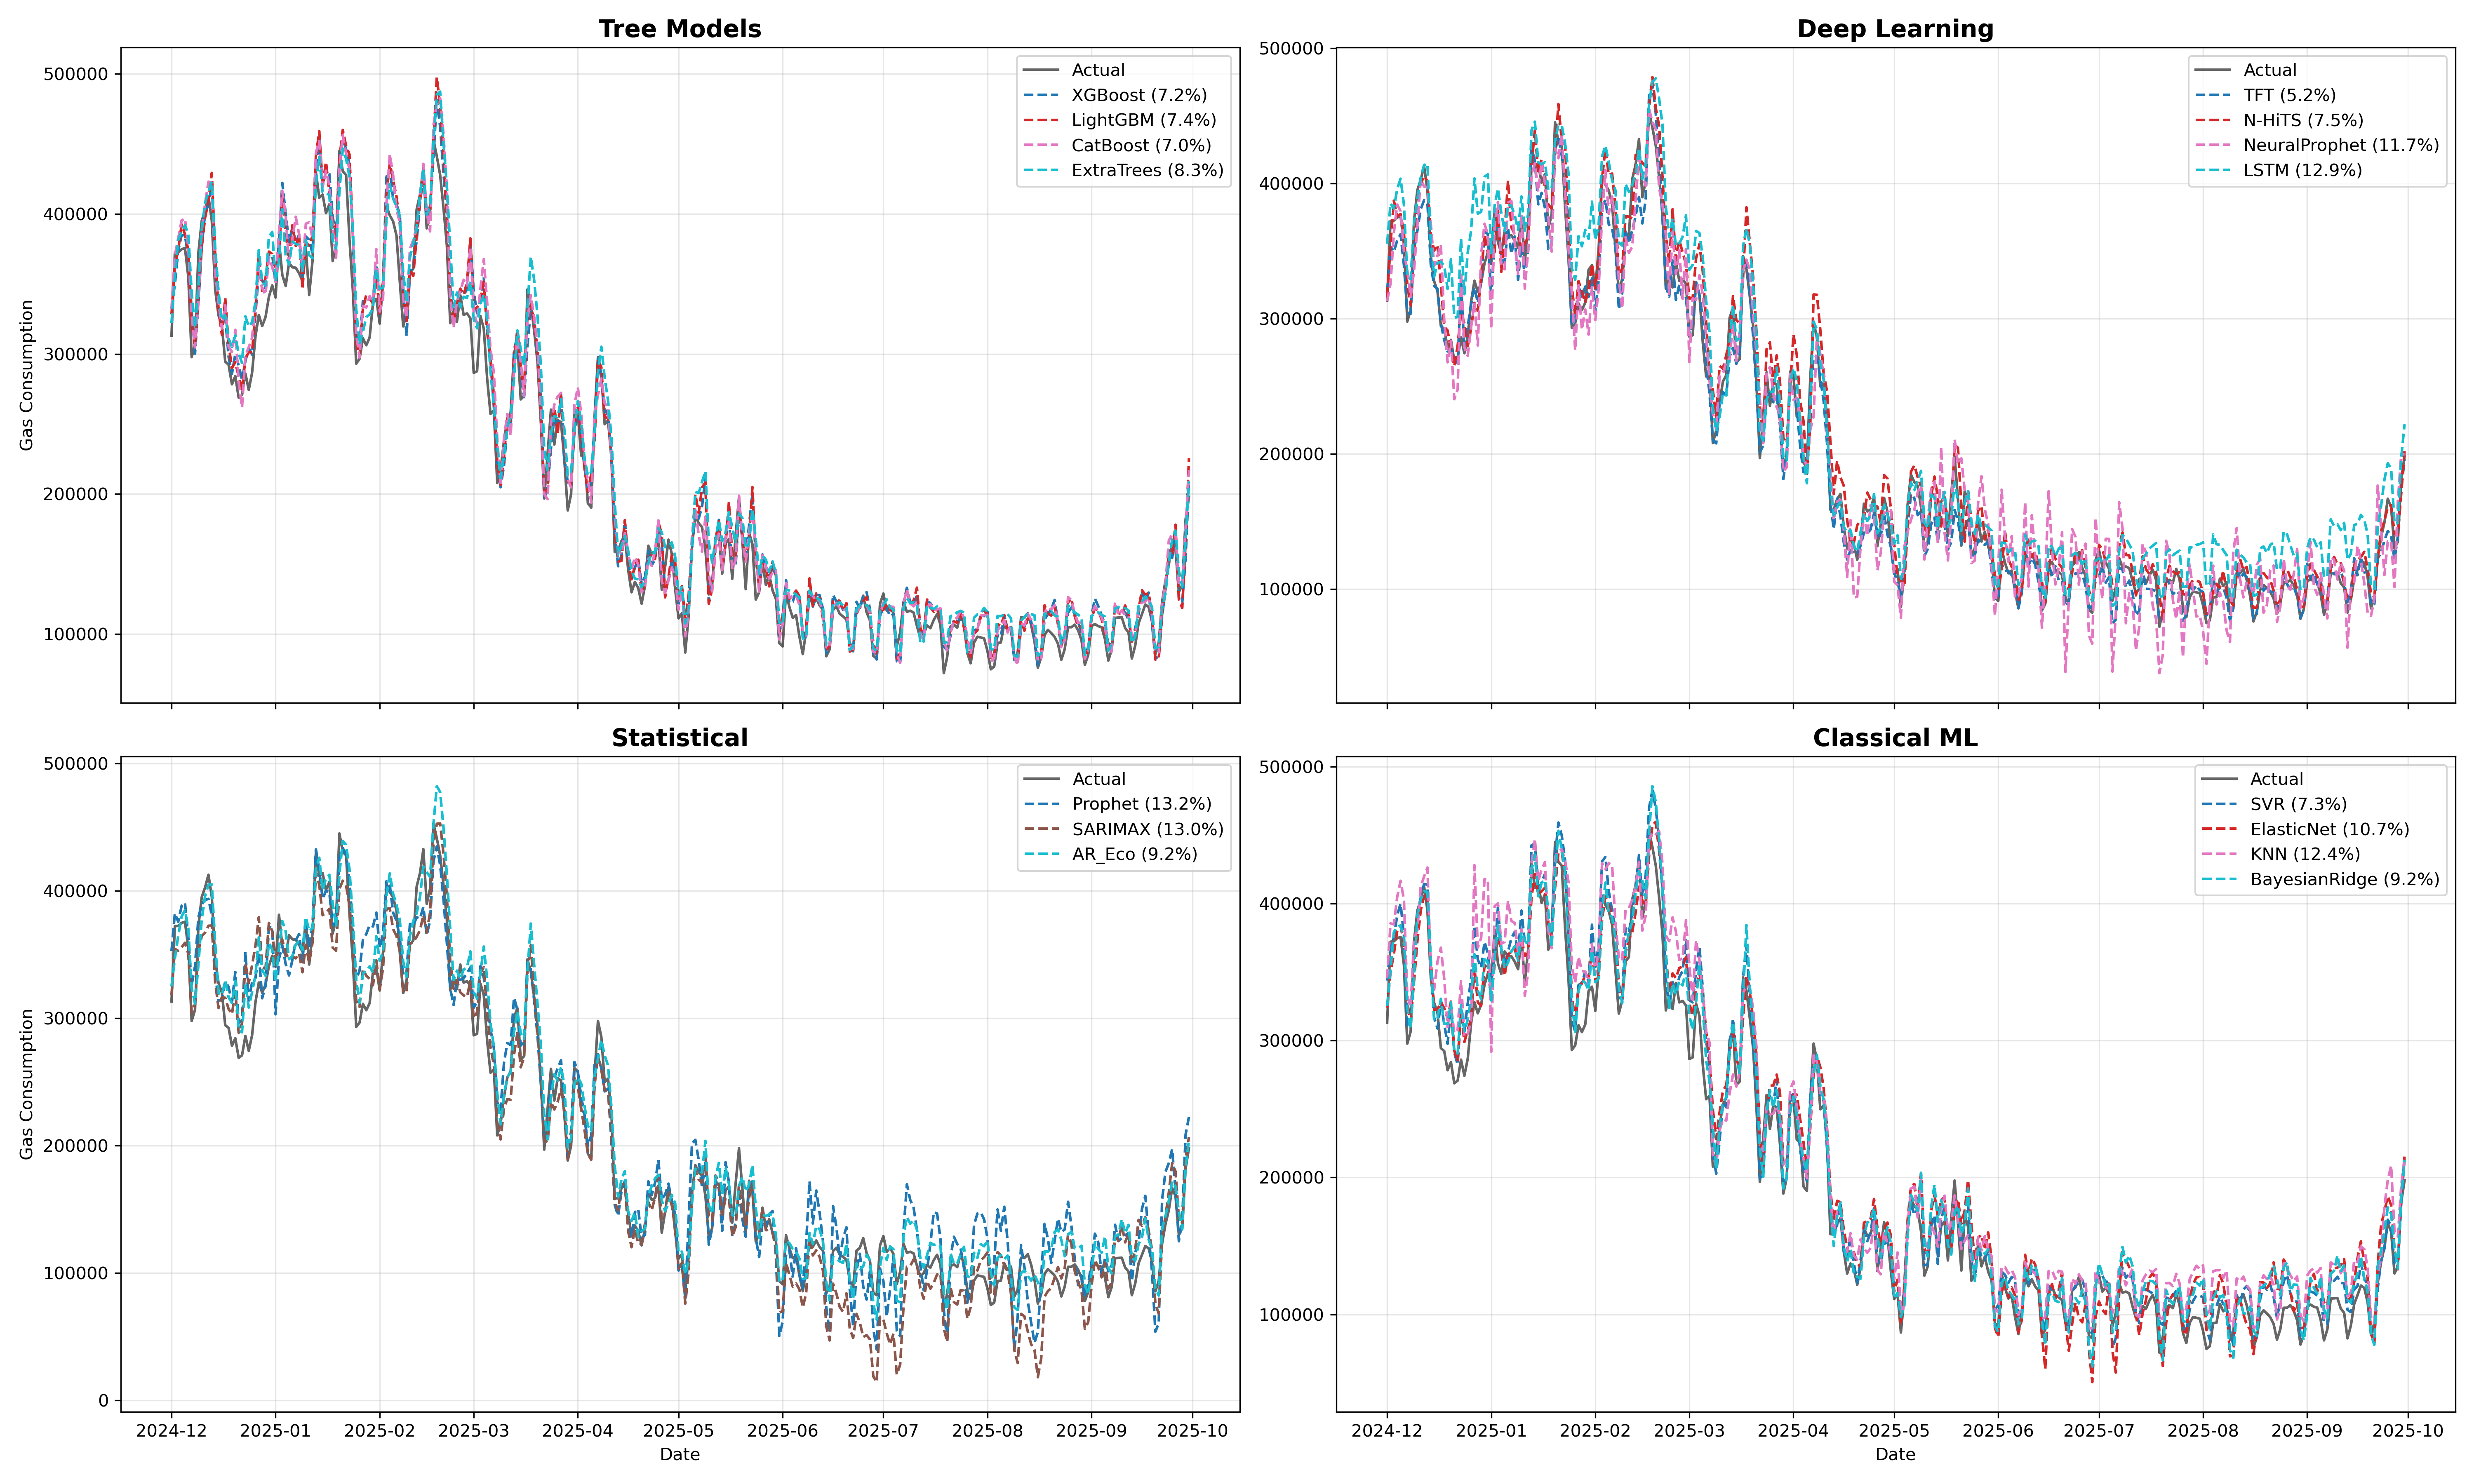
\includegraphics[width=0.95\textwidth]{report_base_models_grouped.png}
\caption{Comparison of base learner predictions grouped by model family (Tree Models, Deep Learning, Statistical, Classical ML) against actual consumption. Deep learning models exhibit the tightest fit to the ground truth.}
\label{fig:base_models_grouped}
\end{figure}

\subsection{Ensemble Optimization Results}
The application of dynamic weighting strategies yielded substantial improvements. Table \ref{tab:ensemble_results} summarizes the performance of different optimization strategies using a 6-week history window, which proved to be optimal in our extended analysis.

\begin{table}[H]
\caption{Comparison of Optimal Ensemble Strategies (6-Week Window)}
\label{tab:ensemble_results}
\centering
\begin{tabular}{lccc}
\toprule
\textbf{Strategy} & \textbf{MAE} & \textbf{RMSE} & \textbf{MAPE (\%)} \\
\midrule
\textbf{Frank-Wolfe (6 weeks, Weighted)} & \textbf{8,235} & \textbf{11,375} & \textbf{4.25} \\
Ensemble Selection (6 weeks, Weighted) & 8,279 & 11,447 & 4.26 \\
Ensemble Selection (6 weeks, Exponential) & 8,202 & 11,260 & 4.26 \\
Frank-Wolfe (6 weeks, Exponential) & 8,221 & 11,345 & 4.27 \\
NNLS (6 weeks, Weighted) & 9,000 & 12,379 & 4.66 \\
\midrule
\textit{Benchmarks:} & & & \\
Best Single Model (N-HiTS) & 10,253 & 13,893 & 5.31 \\
Contextual Bandit (Online) & 10,050 & 13,321 & 5.43 \\
Simple Ensemble Average & 11,723 & 14,897 & 6.74 \\
\bottomrule
\end{tabular}
\end{table}

\begin{itemize}
    \item \textbf{Superiority of Optimization:} The optimized ensemble achieved a MAPE of 4.25\%, reducing the error by more than 1 percentage point relative to the best single model (N-HiTS) and by 2.5 percentage points relative to static averaging.
    \item \textbf{The "Sweet Spot" of Memory:} Our extended analysis identified that a 6-week lookback window provides the optimal balance. Stability increases up to 6 weeks before data drift starts to affect the results. This sensitivity analysis is visualized in Figure \ref{fig:sensitivity}.
    \item \textbf{Validation of "Recency-Weighted" Heuristic:} We explicitly compared our proposed "Recency-Weighted" strategy against a standard exponential decay. The Weighted approach (4.25\%) performed slightly better than Exponential (4.27\%) in the Frank-Wolfe framework, validating the simple heuristic as a robust choice.
    \item \textbf{Method Comparison:} Frank-Wolfe consistently outperformed NNLS (4.66\%). The iterative nature of Frank-Wolfe ($K=500$) acts as an effective regularization against overfitting.
\end{itemize}

\begin{figure}[H]
\centering
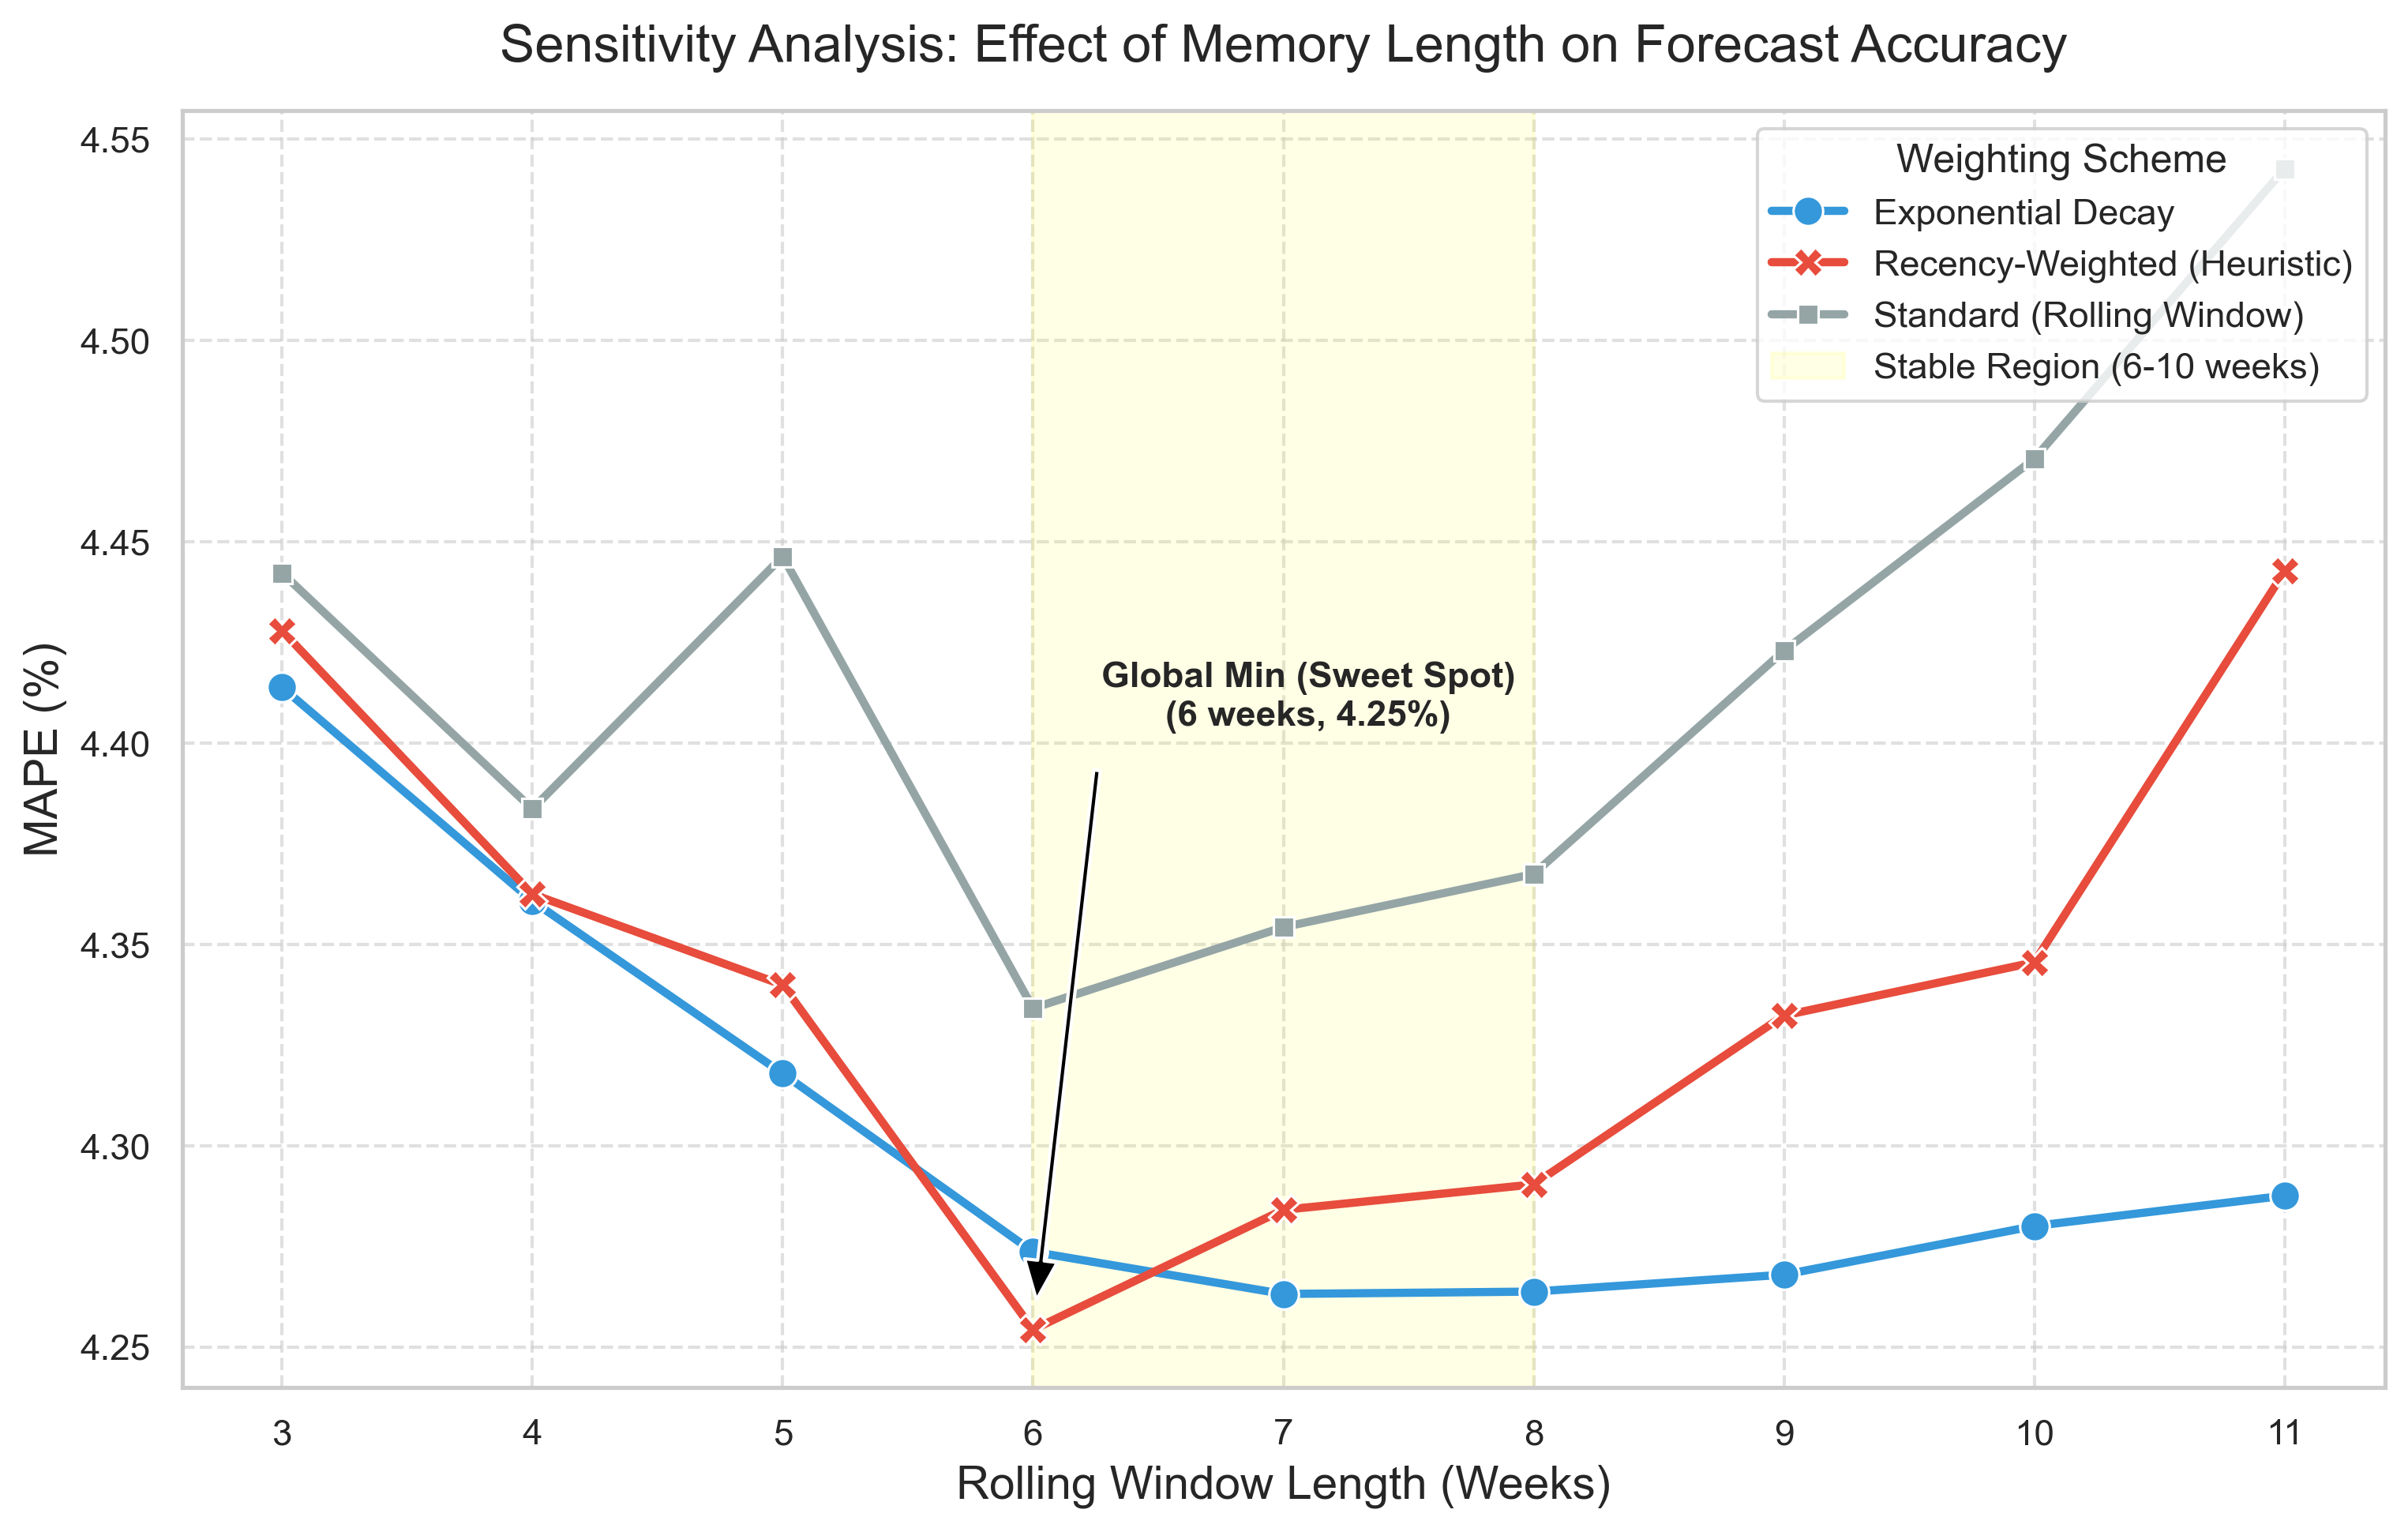
\includegraphics[width=0.8\textwidth]{sensitivity_analysis.png}
\caption{Sensitivity Analysis: Effect of Rolling Window Length on Forecast Accuracy (MAPE) using the Frank-Wolfe optimization. The analysis reveals a robust "sweet spot" around 6 weeks, balancing model stability with adaptability to recent trends.}
\label{fig:sensitivity}
\end{figure}

Figure \ref{fig:weights} illustrates the evolution of weights for the winning strategy. The system dynamically reallocates weights, effectively "hedging" against the failure of any single predictor.

\begin{figure}[H]
\centering
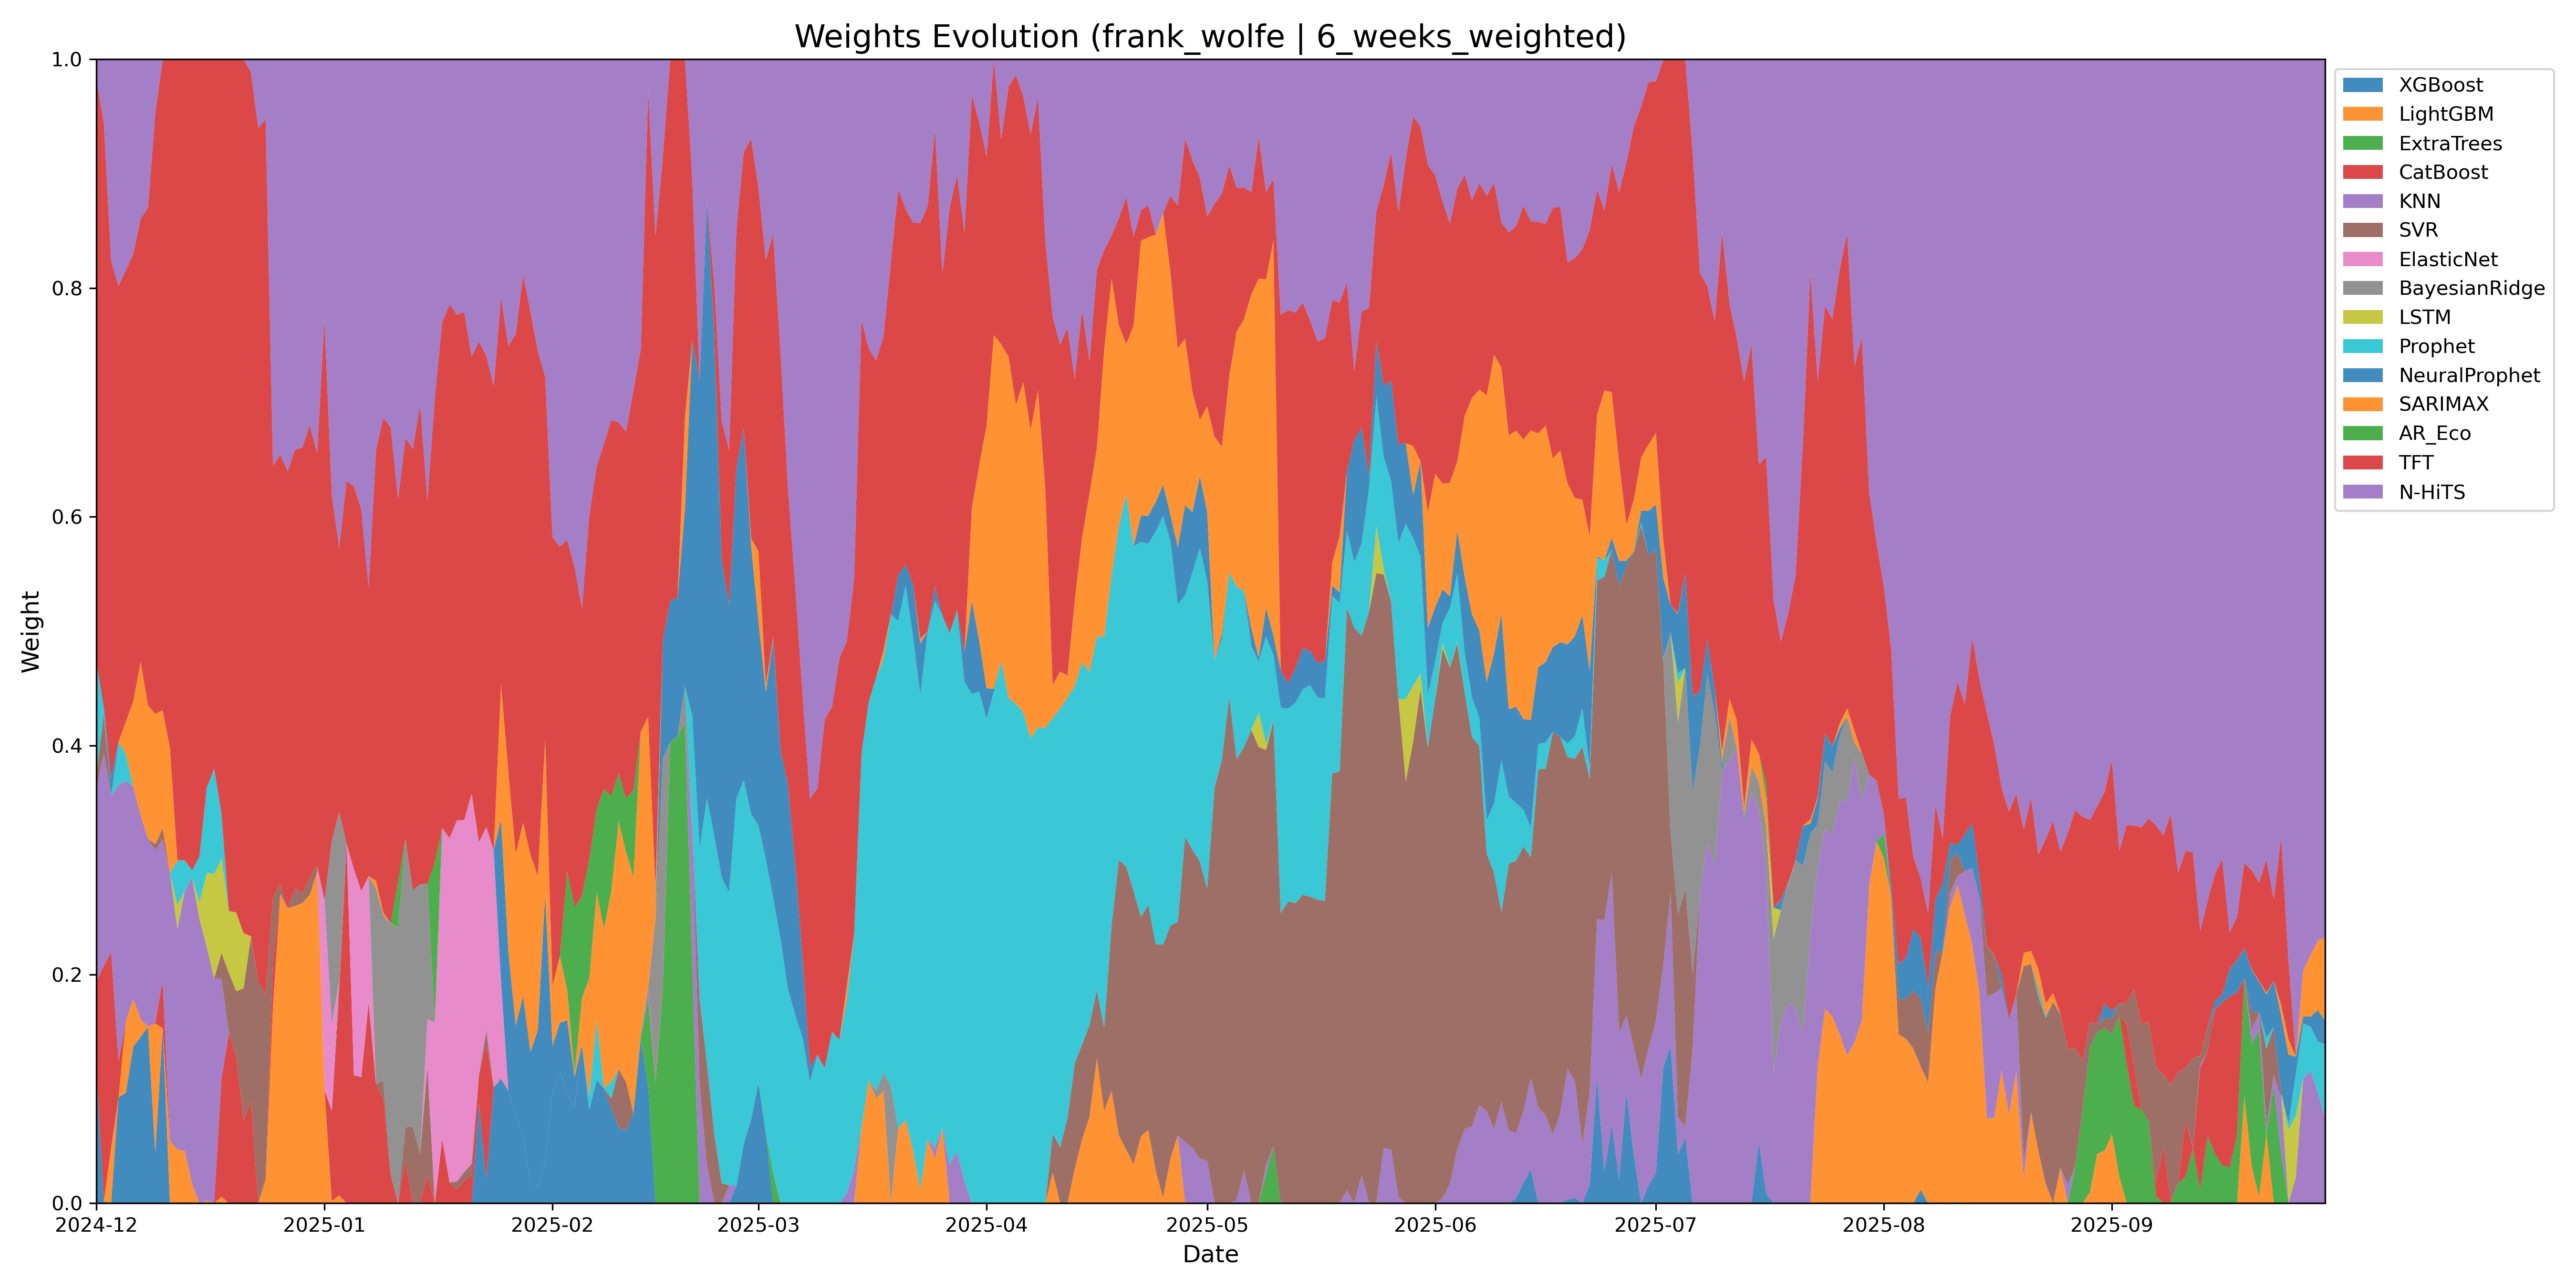
\includegraphics[width=0.95\textwidth]{weights_evolution_frank_wolfe_6_weeks_weighted.png}
\caption{Evolution of model weights over the test period (Frank-Wolfe, 6-week weighted window). The meta-learner actively adapts to changing market conditions by shifting weights between TFT, N-HiTS, and Gradient Boosting models.}
\label{fig:weights}
\end{figure}

To complement the visualization and address the interpretability of the dynamic weight allocation, Table \ref{tab:weights_summary} presents the average weight contribution of the top performing base learners over the test period.
The Frank-Wolfe algorithm inherently promotes sparsity; out of 15 available models, it actively utilizes only a subset, effectively filtering out noise from weaker predictors like KNN or standard Prophet.

\begin{table}[H]
\caption{Average weight allocation ($\bar{w}$) assigned by the Frank-Wolfe optimizer (Recency-Weighted strategy). Models with negligible weights ($< 1\%$) are aggregated.}
\label{tab:weights_summary}
\centering
\begin{tabular}{llc}
\toprule
\textbf{Model Family} & \textbf{Base Learner} & \textbf{Avg. Weight (\%)} \\
\midrule
\multirow{3}{*}{Deep Learning} & N-HiTS & 29.3\% \\
 & TFT & 27.5\% \\
 & NeuralProphet & 3.6\% \\
\midrule
\multirow{4}{*}{Tree-Based} & LightGBM & 3.1\% \\
 & XGBoost & 1.4\% \\
 & ExtraTrees & 1.3\% \\
 & CatBoost & 1.2\% \\
\midrule
\multirow{7}{*}{Statistical/Other} & SVR & 10.0\% \\
 & Prophet & 9.2\% \\
 & SARIMAX & 5.7\% \\
 & KNN & 4.7\% \\
 & BayesianRidge & 1.5\% \\
 & ElasticNet & 1.0\% \\
 & \textit{Others (aggregated)} & 0.6\% \\
\bottomrule
\end{tabular}
\end{table}

\subsection{Statistical Significance Testing}
To determine whether the observed improvements in forecast accuracy are statistically significant or merely artifacts of stochastic variation, we conducted rigorous non-parametric testing mandated for time-series comparisons.

\subsubsection{Diebold-Mariano Test}
We employed the Diebold-Mariano (DM) test to perform a pairwise comparison between the proposed Frank-Wolfe (Weighted) strategy and the second-best alternative, Ensemble Selection. The null hypothesis $H_0$ states that both forecasting methods have equal predictive accuracy.
The test statistic was calculated based on the Mean Absolute Error (MAE) differential series:
\begin{equation}
    d_t = |e_{1,t}| - |e_{2,t}|
\end{equation}
where $e_{1,t}$ and $e_{2,t}$ denote the forecast errors of the primary model (Frank-Wolfe) and the benchmark model (Ensemble Selection) at time $t$, respectively. The results yielded a DM statistic of $-1.11$ with a $p$-value of $0.2669$. Consequently, we fail to reject the null hypothesis at the 5\% significance level. This statistical equivalence supports our argument in the Discussion section: while Frank-Wolfe does not statistically outperform Ensemble Selection in raw accuracy, its preference is justified by computational stability and \textit{sparsity} properties rather than marginal error reduction.

\subsubsection{Friedman Test and Pairwise Significance}
To rigorously assess the hierarchy of methods, we followed the methodology recommended by \citep{ref_demsar} for comparing algorithms over multiple datasets. We employed the non-parametric Friedman test to detect global differences, followed by a Nemenyi post-hoc analysis for pairwise comparisons. Furthermore, to assess the specific significance of the improvement of the proposed method over the best baseline, we utilized the Diebold-Mariano test \citep{ref_dm_test}.
The Friedman test rejected the null hypothesis of equal performance ($p < 0.001$).
Table \ref{tab:significance} synthesizes the pairwise statistical significance between the proposed Frank-Wolfe ensemble and key benchmarks.

\begin{table}[H]
\caption{Pairwise statistical significance (Nemenyi Test, $\alpha=0.05$). $\checkmark$ indicates a significant difference, $-$ indicates no significant difference.}
\label{tab:significance}
\centering
\begin{tabular}{lccc}
\toprule
\textbf{Comparison Pair (A vs. B)} & \textbf{p-value} & \textbf{Significant?} & \textbf{Winner} \\
\midrule
Frank-Wolfe vs. Ensemble Selection & 0.998 & $-$ & Draw \\
Frank-Wolfe vs. N-HiTS (Best Single) & $< 0.01$ & $\checkmark$ & Frank-Wolfe \\
Frank-Wolfe vs. XGBoost & $< 0.001$ & $\checkmark$ & Frank-Wolfe \\
Frank-Wolfe vs. Simple Averaging & $< 0.001$ & $\checkmark$ & Frank-Wolfe \\
N-HiTS vs. XGBoost & $< 0.05$ & $\checkmark$ & N-HiTS \\
\bottomrule
\end{tabular}
\end{table}

The results confirm that while the difference between the two sophisticated ensemble methods (FW and ES) is not statistically significant, both form a statistically superior cluster compared to individual state-of-the-art models and simple averaging.

\subsubsection{Ablation Study}
To isolate the contribution of the proposed optimization framework, we performed an ablation study comparing the full Frank-Wolfe ensemble against simplified baselines. Table \ref{tab:ablation} demonstrates the incremental gain from each component of the proposed methodology.

% already set
% \newcolumntype{L}[1]{>{\raggedright\let\newline\\\arraybackslash\hspace{0pt}}p{#1}}

\begin{table}[H]
\caption{Ablation study quantifying the impact of ensemble components on forecast accuracy (MAPE).}
\label{tab:ablation}
\centering
\small % Trochu menší písmo pro lepší estetiku
\setlength{\tabcolsep}{4pt} % Optimalizované mezery
\begin{tabular}{L{2.5cm} L{5.5cm} c L{3.5cm}}
\toprule
\textbf{Component Level} & \textbf{Method Description} & \textbf{MAPE (\%)} & \textbf{Rel. Improvement} \\
\midrule
1. Baseline & Best Single Model (N-HiTS) & 5.31\% & - \\
2. Naïve Comb. & Simple Ensemble Average (Mean) & 6.74\% & -26.9\% (Deterioration) \\
3. Standard Opt. & NNLS (Rolling Window) & 4.60\% & +13.4\% \\
4. Dynamic Opt. & Frank-Wolfe (Rolling Window) & 4.33\% & +18.5\% \\
\textbf{5. Proposed} & \textbf{Frank-Wolfe + Temporal Weighting} & \textbf{4.25\%} & \textbf{+20.0\%} \\
\bottomrule
\end{tabular}
\end{table}

The results indicate that simple averaging actually deteriorates performance due to the inclusion of weaker learners. The introduction of convex optimization (NNLS) restores performance, but the significant leap in accuracy is achieved only by making the optimization dynamic (Frank-Wolfe) and context-aware (Temporal Weighting).

%%%%%%%%%%%%%%%%%%%%%%%%%%%%%%%%%%%%%%%%%%
\section{Discussion}

The empirical results substantiate the hypothesis that the application of operations research methods to the weighting of machine learning predictions offers a transparent and controllable mechanism for improving forecast accuracy. The 6-week weighted window appears to serve as a robust heuristic for the Czech gas market.

\textbf{Stability vs. Accuracy:} Although the difference in accuracy (0.01 p.p.) between Frank-Wolfe (MAPE 4.25\%) and Ensemble Selection (MAPE 4.26\%) is statistically negligible (Diebold-Mariano test, $p = 0.2669$), we argue that Frank-Wolfe is the superior choice for production environments. A granular inspection of the weight evolution (Figure \ref{fig:weights}) reveals a critical operational difference rooted in the mathematical nature of the algorithms.

Ensemble Selection is a discrete, greedy algorithm that selects models from a finite set. This leads to step-wise weight changes, where the algorithm suddenly shifts confidence from one model to another based on marginal short-term gains. In contrast, Frank-Wolfe operates in a continuous space on the simplex. As observed during the experimental transition periods, Frank-Wolfe produces smooth, gradual weight reallocations, avoiding the "bang-bang" behavior typical of greedy heuristics. As noted by \citep{ref_fw_jaggi}, this property of sparse convex optimization provides better stability guarantees than greedy heuristics in high-dimensional spaces. For a market operator, this smoothness minimizes the operational risk and transaction costs associated with abrupt daily shifts in trading strategies, justifying the preference for the convex optimization approach despite the parity in raw accuracy. This observation aligns with the "forecast combination puzzle" discussed by \citep{ref_elliott}, where sophisticated weighting schemes often show only marginal accuracy gains over simple averages due to estimation noise. However, our results demonstrate that the primary value of convex optimization lies not merely in error reduction, but in the \textit{stability} and \textit{sparsity} of the solution, which are critical for risk-averse market operators.

\textbf{Interpretability:} Unlike black-box AutoML solutions, our Convex Weight Optimization framework maintains high interpretability. The weights $\mathbf{w}$ directly represent the confidence in each underlying model (e.g., "today we trust N-HiTS 40\% and XGBoost 60\%"), effectively treating the forecast as an investment portfolio.

It is worth noting that the Prophet model was included primarily as a representative baseline for Generalized Additive Models (GAMs), distinct from the intensively tuned ensemble components. The observed performance difference relative to N-HiTS suggests that the default additive assumptions of standard GAMs may require more extensive manual feature engineering to fully capture the heteroscedastic nature of gas demand. In contrast, the gradient boosting and deep learning approaches demonstrated a stronger capacity to autonomously extract these non-linear dependencies from the same input data.

%%%%%%%%%%%%%%%%%%%%%%%%%%%%%%%%%%%%%%%%%%
\section{Conclusions}

This study reformulated the daily natural gas consumption forecasting task from a model-selection problem to a constrained convex optimization problem on the unit simplex. By applying the Frank-Wolfe algorithm, we established a rigorous meta-learning framework that guarantees convergence to a global optimum for convex loss functions, addressing the lack of theoretical grounding in standard heuristic ensembles.

\subsection{Synthesis of Empirical and Theoretical Findings}
Our results confirm the superiority of dynamic convex optimization over both state-of-the-art individual models and static ensemble techniques. The proposed framework achieved a Mean Absolute Percentage Error (MAPE) of 4.25\%, representing a statistically significant improvement over the best single deep learning model (N-HiTS, 5.31\%) and the simple ensemble average (6.74\%). 

Crucially, the ablation study quantified the sources of this improvement:
\begin{itemize}
    \item \textbf{Dynamic Adaptation:} Transitioning from static weights (NNLS, MAPE 4.66\%) to time-varying weights (Frank-Wolfe) yielded a relative accuracy gain of approximately 9\%, confirming that adapting to concept drift is as critical as model selection.
    \item \textbf{Physical Grounding of Hyperparameters:} We demonstrated that the optimal look-back window of 6 weeks is not arbitrary but reflects the quasi-stationarity period of seasonal consumption patterns. Similarly, the "Recency-Weighted" heuristic ($\omega_{high}=3$) aligns with the physical inertia of synoptic weather systems (3--5 days) in Central Europe, acting as an effective Bayesian prior for the optimization process.
    \item \textbf{Algorithmic Stability:} While the Diebold-Mariano test ($p=0.2669$) indicated parity in raw accuracy between Frank-Wolfe and the greedy Ensemble Selection method, the convex approach is strictly preferred for operational deployment. Unlike the discrete selection of greedy algorithms, Frank-Wolfe operates in continuous space, producing sparse and stable weight vectors that minimize transaction costs in decision-making.
\end{itemize}

\subsection{Limitations and Future Research Directions}
The validity of these findings is bound by the specific regulatory and climatic context of the Czech Republic and the use of ERA5 reanalysis data. Operational implementation would introduce additional uncertainty stemming from real-time Numerical Weather Prediction (NWP) errors. Furthermore, the computational cost of retraining deep learning base learners remains a bottleneck for high-frequency updates.

Future research will extend this framework in four directions:
\begin{itemize}
    \item \textbf{Data Availability and Robustness:} The study is validated on a test set spanning a single gas year (2024--2025). While this captures a complete seasonal cycle (heating vs. non-heating transitions), rigorous testing on multiple years is identified as a necessary step to assess robustness against long-term climatic anomalies (e.g., extremely mild winters).
    \item \textbf{Online Learning:} Replacing the batch-based rolling window with fully online algorithms, such as Weighted Linear Bandits, to reduce computational complexity to $\mathcal{O}(1)$ per step.
    \item \textbf{Probabilistic Forecasting:} Generalizing the loss function from MSE to Pinball Loss (Quantile Regression) to generate conformal prediction intervals, which are essential for risk-aware bidding strategies.
    \item \textbf{Multi-Energy Coupling:} Incorporating renewable energy generation (solar, wind) as exogenous variables to capture the increasing cross-commodity correlations in modern energy grids.
\end{itemize}

%%%%%%%%%%%%%%%%%%%%%%%%%%%%%%%%%%%%%%%%%%
\vspace{6pt} 

%%%%%%%%%%%%%%%%%%%%%%%%%%%%%%%%%%%%%%%%%%
\authorcontributions{Conceptualization, J.J. and V.V.; methodology, V.V.; software, V.V.; validation, J.J. and V.V.; formal analysis, V.V.; writing---original draft preparation, V.V.; writing---review and editing, J.J. All authors have read and agreed to the published version of the manuscript.}

\funding{The author gratefully acknowledges support from the Internal Grant Agency, Faculty of Informatics and Statistics, Prague University of Economics and Business (Project No. F4/10/2024).}

%\institutionalreview{Not applicable.}

%\informedconsent{Not applicable.}

\dataavailability{Publicly available datasets were analyzed in this study. The data can be found at \url{https://www.ote-cr.cz/} and \url{https://open-meteo.com/en/docs/historical-weather-api}.} 

\acknowledgments{We thank the anonymous referees for their time and comments.}

\conflictsofinterest{The authors declare no conflict of interest.} 

%%%%%%%%%%%%%%%%%%%%%%%%%%%%%%%%%%%%%%%%%%
\begin{adjustwidth}{-\extralength}{0cm}
\reftitle{References}
\isAPAStyle{}{%
\begin{thebibliography}{999}

\bibitem[\protect\citeauthoryear{Boyd and Vandenberghe}{{2004}}]{ref_boyd}
Boyd, S., \& Vandenberghe, L. (2004). \textit{Convex Optimization}. Cambridge University Press.

\bibitem[\protect\citeauthoryear{Caruana et al.}{{2004}}]{ref_caruana}
Caruana, R., Niculescu-Mizil, A., Crew, G., \& Ksikes, A. (2004). Ensemble selection from libraries of models. In \textit{Proceedings of the 21st International Conference on Machine Learning} (p. 18). ACM.

\bibitem[\protect\citeauthoryear{Challu et al.}{{2023}}]{ref_nhits}
Challu, C., Olivares, K. G., Oreshkin, B. N., Ramirez, F. G., Canseco, M. M., \& Dubrawski, A. (2023). N-HiTS: Neural Hierarchical Interpolation for Time Series Forecasting. \textit{Proceedings of the AAAI Conference on Artificial Intelligence}, 37, 6989--6997.

\bibitem[\protect\citeauthoryear{Chen and Guestrin}{{2016}}]{ref_xgboost}
Chen, T., \& Guestrin, C. (2016). XGBoost: A Scalable Tree Boosting System. In \textit{Proceedings of the 22nd ACM SIGKDD International Conference on Knowledge Discovery and Data Mining} (pp. 785--794). ACM.

\bibitem[\protect\citeauthoryear{De Myttenaere et al.}{{2016}}]{ref_mape_theory}
De Myttenaere, A., Golden, B., Le Grand, B., \& Rossi, F. (2016). Mean absolute percentage error for regression models.
\textit{Neurocomputing}, 192, 38--48.

\bibitem[\protect\citeauthoryear{Dem{\v{s}}ar}{{2006}}]{ref_demsar}
Dem{\v{s}}ar, J. (2006). Statistical comparisons of classifiers over multiple data sets.
\textit{Journal of Machine Learning Research}, 7, 1--30.

\bibitem[\protect\citeauthoryear{Diebold and Mariano}{{2002}}]{ref_dm_test}
Diebold, F. X., \& Mariano, R. S. (2002). Comparing predictive accuracy.
\textit{Journal of Business \& Economic Statistics}, 20(1), 134--144.

\bibitem[\protect\citeauthoryear{Dudek}{{2021}}]{Dudek2021}
Dudek, G. (2021). A Comprehensive Study of Random Forest for Short-Term Load Forecasting. \textit{Energies}, 14(21), 6922. 
%\url{https://doi.org/10.3390/en14216922}

\bibitem[\protect\citeauthoryear{Elliott and Liao}{{2025}}]{ref_elliott}
Elliott, G., \& Liao, J. (2025). Combining Forecasts-On Why Averaging beats Optimal Linear Weights.
\textit{Manuscript, University of California, San Diego}.

\bibitem[\protect\citeauthoryear{Frank and Wolfe}{{1956}}]{ref_fw_orig}
Frank, M., \& Wolfe, P. (1956). An algorithm for quadratic programming. \textit{Naval Research Logistics Quarterly}, 3(1-2), 95--110.

\bibitem[\protect\citeauthoryear{Jaggi}{{2013}}]{ref_fw_jaggi}
Jaggi, M. (2013). Revisiting Frank-Wolfe: Projection-Free Sparse Convex Optimization. In \textit{Proceedings of the 30th International Conference on Machine Learning} (pp. 427--435). PMLR.

\bibitem[\protect\citeauthoryear{Ke et al.}{{2017}}]{ref_lgbm}
Ke, G., Meng, Q., Finley, T., Wang, T., Chen, W., Ma, W., Ye, Q., \& Liu, T.-Y. (2017). LightGBM: A Highly Efficient Gradient Boosting Decision Tree. \textit{Advances in Neural Information Processing Systems}, 30.

\bibitem[\protect\citeauthoryear{Li and Sun}{{2021}}]{ref_li_emlp}
Li, F., \& Sun, M. (2021). EMLP: short-term gas load forecasting based on ensemble multilayer perceptron with adaptive weight correction.
\textit{Mathematical Biosciences and Engineering}, 18(2), 1590--1608.

\bibitem[\protect\citeauthoryear{Lim et al.}{{2021}}]{ref_tft}
Lim, B., Arik, S. O., Loeff, N., \& Pfister, T. (2021). Temporal Fusion Transformers for Interpretable Multi-horizon Time Series Forecasting. \textit{International Journal of Forecasting}, 37(4), 1748--1764.

\bibitem[\protect\citeauthoryear{Marziali et al.}{{2021}}]{ref_marziali}
Marziali, A., Fabbiani, E., \& De Nicolao, G. (2021). Ensembling methods for countrywide short-term forecasting of gas demand.
\textit{International Journal of Oil, Gas and Coal Technology}, 26(2), 184--201.

\bibitem[\protect\citeauthoryear{Nalcaci et al.}{{2019}}]{ref_mdpi_energies_1}
Nalcaci, G., Ozmen, A., \& Weber, G. W. (2019). Long-term natural gas consumption forecasting with MARS and CMARS models. \textit{Energies}, 12(10), 1989.

\bibitem[\protect\citeauthoryear{Oliveira and Torgo}{{2014}}]{ref_oliveira}
Oliveira, M., \& Torgo, L. (2014). Ensembles for Time Series Forecasting. \textit{Proceedings of the Asian Conference on Machine Learning}, 39, 360--370.

\bibitem[\protect\citeauthoryear{OTE}{{2025}}]{ref_ote}
OTE, a.s. (2025). \textit{Metodika teplotního přepočtu TDD pro rok 2023}. Available online: \url{https://www.ote-cr.cz/} (accessed on 12 December 2025).

\bibitem[\protect\citeauthoryear{Panapakidis~and Dagoumas}{{2017}}]{ref_panapakidis}
Panapakidis, I. P., \& Dagoumas, A. S. (2017). Day-ahead natural gas demand forecasting based on the combination of wavelet transform and ANFIS/genetic algorithm/neural network model.
\textit{Energy}, 118, 231--245.

\bibitem[\protect\citeauthoryear{Paszke et al.}{{2019}}]{ref_pytorch}
Paszke, A., Gross, S., Massa, F., Lerer, A., Bradbury, J., Chanan, G., Killeen, T., Lin, Z., Gimelshein, N., Antiga, L., et al. (2019). PyTorch: An Imperative Style, High-Performance Deep Learning Library. \textit{Advances in Neural Information Processing Systems}, 32.

\bibitem[\protect\citeauthoryear{Pedregosa et al.}{{2011}}]{ref_scikit}
Pedregosa, F., Varoquaux, G., Gramfort, A., Michel, V., Thirion, B., Grisel, O., Blondel, M., Prettenhofer, P., Weiss, R., Dubourg, V., et al. (2011). Scikit-learn: Machine Learning in Python. \textit{Journal of Machine Learning Research}, 12, 2825--2830.

\bibitem[\protect\citeauthoryear{Poto{\v{c}}nik et al.}{{2014}}]{ref_potocnik}
Poto{\v{c}}nik, P., Soldo, B., {\v{S}}imunovi{\'c}, G., {\v{S}}ari{\'c}, T., Jeromen, A., \& Govekar, E. (2014). Comparison of static and adaptive models for short-term residential natural gas forecasting in Croatia.
\textit{Applied Energy}, 129, 94--103.

\bibitem[\protect\citeauthoryear{Prokhorenkova et al.}{{2018}}]{ref_catboost}
Prokhorenkova, L., Gusev, G., Vorobev, A., Dorogush, A. V., \& Gulin, A. (2018). CatBoost: Unbiased Boosting with Categorical Features. \textit{Advances in Neural Information Processing Systems}, 31.

\bibitem[\protect\citeauthoryear{Sharma et al.}{{2021}}]{ref_sharma}
Sharma, V., Cali, {\"U}., Sardana, B., Kuzlu, M., Banga, D., \& Pipattanasomporn, M. (2021). Data-driven short-term natural gas demand forecasting with machine learning techniques.
\textit{Journal of Petroleum Science and Engineering}, 206, 108979.

\bibitem[\protect\citeauthoryear{Smajla et al.}{{2023}}]{ref_smajla}
Smajla, I., Vulin, D., \& Sedlar, D. K. (2023). Short-term forecasting of natural gas consumption by determining the statistical distribution of consumption data.
\textit{Energy Reports}, 10, 2352--2360.

\bibitem[\protect\citeauthoryear{Svoboda et al.}{{2021}}]{ref_svoboda}
Svoboda, R., Kotik, V., \& Platos, J. (2021). Short-term natural gas consumption forecasting from long-term data collection.
\textit{Energy}, 218, 119430.

\bibitem[\protect\citeauthoryear{Taylor and Letham}{{2018}}]{ref_prophet}
Taylor, S. J., \& Letham, B. (2018). Forecasting at Scale. \textit{The American Statistician}, 72(1), 37--45.

\bibitem[\protect\citeauthoryear{Wang et al.}{{2020}}]{ref_mdpi_math_1}
Wang, J., Du, Y., \& Wang, J. (2020). LSTM based long-term energy consumption forecasting with periodicity. \textit{Mathematics}, 8(12), 2139.

\bibitem[\protect\citeauthoryear{Wu and Levinson}{{2021}}]{ref_wu_review}
Wu, H., \& Levinson, D. (2021). The Ensemble Approach to Forecasting: A Review and Synthesis. \textit{Transportation Research Part C: Emerging Technologies}, 132, 103357.

\bibitem[\protect\citeauthoryear{Zhang et al.}{{2022}}]{ref_mdpi_energies_2}
Zhang, Y., Li, J., \& Li, X. (2022). Ensemble forecasting of natural gas consumption using dynamic weighting. \textit{Energies}, 15(3), 882.

\bibitem[\protect\citeauthoryear{Zhao et al.}{{2024}}]{ref_zhao}
Zhao, M., Guo, G., Fan, L., Han, L., Yu, Q., \& Wang, Z. (2024). Short-term natural gas load forecasting based on EL-VMD-Transformer-ResLSTM.
\textit{Scientific Reports}, 14(1), 20343.

\bibitem[\protect\citeauthoryear{Zippenfenig}{{2023}}]{ref_openmeteo}
Zippenfenig, P. (2023). Open-Meteo.com Weather API [Computer software]. Zenodo. \url{https://doi.org/10.5281/ZENODO.7970649}

\end{thebibliography}
}
\PublishersNote{}
\end{adjustwidth}

%%%%%%%%%%%%%%%%%%%%%%%%%%%%%%%%%%%%%%%%%%

\end{document}
